\documentclass[12pt,a4paper,titlepage]{article} 
\usepackage[utf8]{inputenc}
\usepackage[spanish]{babel}
\usepackage{graphicx}
\usepackage{booktabs}
\usepackage{geometry}
\usepackage{longtable}
\usepackage{amssymb}
\graphicspath{ {./} }
\geometry{a4paper, margin=2.5cm}

\title{\textbf{Planificación Ciclo 1}}
\author{
    \textbf{Grupo 2:} \\
    Guillermo Guhl Arruabarrena \\
    Daniel Gomarín Ruesga \\
    Marcos Romero Villodres \\
    Carlos Sobrino Martin \\
    Javier Pozuelo Ruiz
}
\date{}

\begin{document}

\maketitle

% Índice
\tableofcontents
\vspace{1cm}

% --- CÓDIGO PARA AÑADIR LA IMAGEN ---
% Para que se muestre, quita el símbolo % de las siguientes 6 líneas 
% y asegúrate de que el nombre del archivo coincida con el tuyo.
%
% \begin{figure}[htbp]
%     \centering
%     \includegraphics[width=\textwidth]{tu_imagen_gantt.png} 
%     \caption{Diagrama de Gantt del Ciclo 1.}
%     \label{fig:diagrama_gantt}
% \end{figure}
% ------------------------------------

\section{Explicación del Diagrama de Gantt}

El diagrama ha sido elaborado usando la funcionalidades disponibles en ClickUp. El objetivo vincular las tareas al diagrama de Gantt establecer las estimaciones
y registrar el tiempo que invertimos en las distintas tareas de manera unificada. Lamentablmente el poder extraer la información en formato pdf requiere de una suscripción de pago
por lo tanto se ha optado por incluir una captura de pantalla.


\begin{figure}[htbp]
    \centering
    % Cambia "nombre_de_tu_imagen.png" por el nombre real de tu archivo
    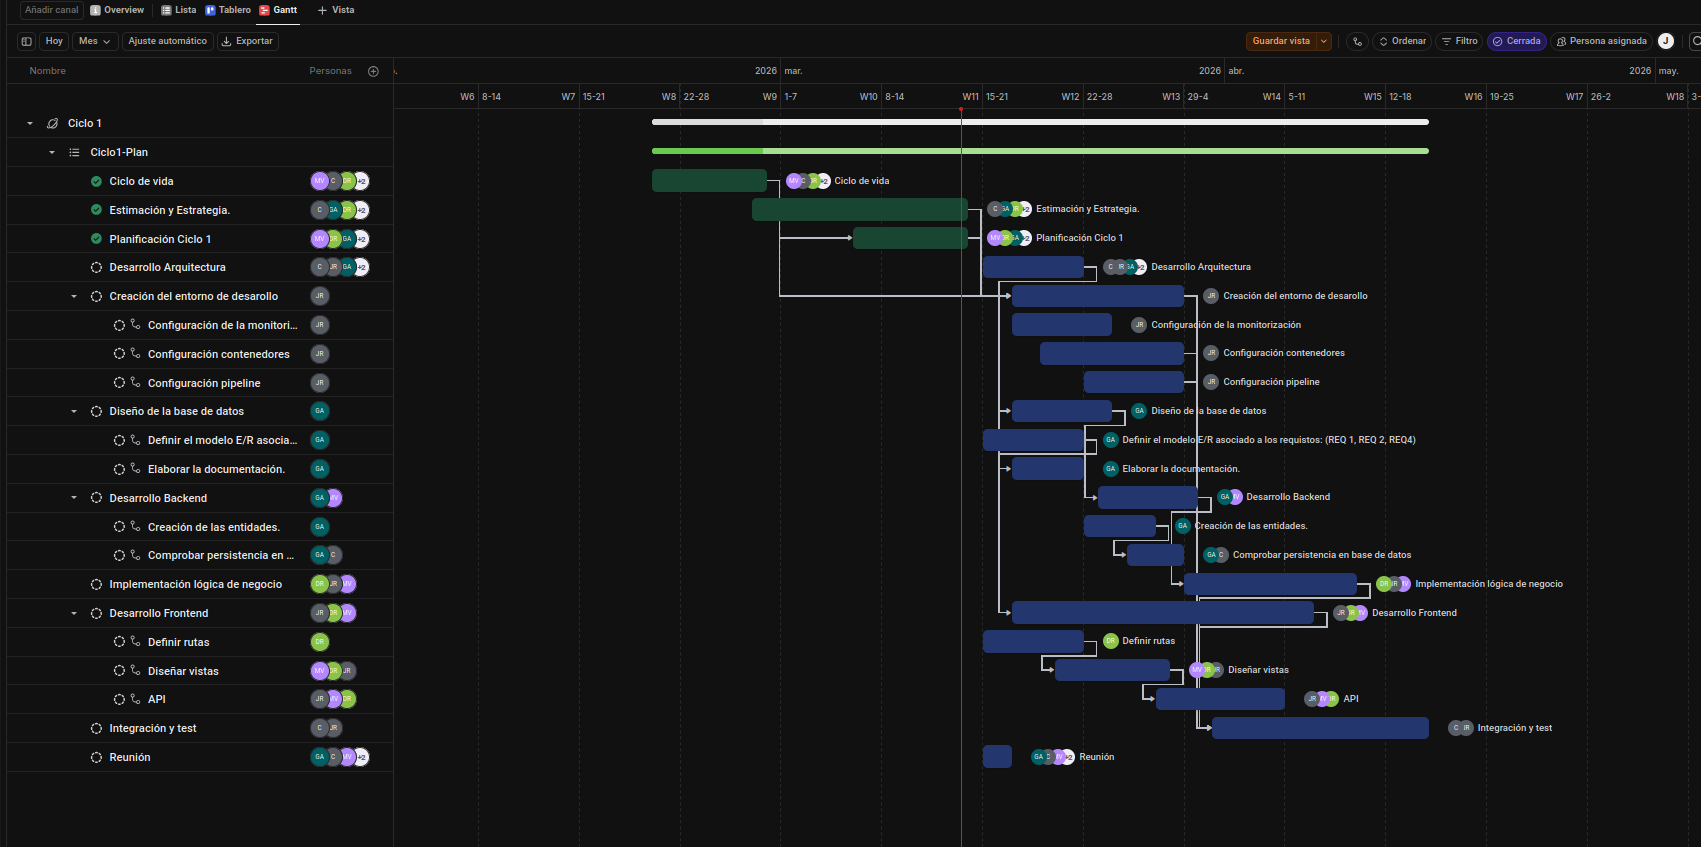
\includegraphics[width=\textwidth]{Diagrama-Gant.png} 
    \caption{Diagrama de Gantt del Ciclo 1.}
    \label{fig:diagrama_gantt}
\end{figure}

\begin{itemize}
    \item \textbf{Ciclo de vida}: Duración de 2 semanas. Asignada a: Marcos Romero Villodres, Carlos Sobrino Martin, Daniel Gomarín Ruesga, Guillermo Guhl Arruabarrena, Javier Pozuelo Ruiz.
    \item \textbf{Estimación y Estrategia.}: Duración de 2 semanas. Asignada a: Carlos Sobrino Martin, Guillermo Guhl Arruabarrena, Daniel Gomarín Ruesga, Marcos Romero Villodres, Javier Pozuelo Ruiz.
    \item \textbf{Planificación Ciclo 1}: Duración de 1 semana. Asignada a: Marcos Romero Villodres, Daniel Gomarín Ruesga, Guillermo Guhl Arruabarrena, Carlos Sobrino Martin, Javier Pozuelo Ruiz.
    \item \textbf{Desarrollo Arquitectura}: Duración de 1 semana. Asignada a: Carlos Sobrino Martin, Javier Pozuelo Ruiz, Guillermo Guhl Arruabarrena, Marcos Romero Villodres, Daniel Gomarín Ruesga.
    
    \item \textbf{Creación del entorno de desarrollo}: Duración de 2 semanas. Asignada a: Javier Pozuelo Ruiz. Esta tarea principal se desglosa en:
    \begin{itemize}
        \item \textbf{Configuración de la monitorización}: Duración de 1 semana. Asignada a: Javier Pozuelo Ruiz.
        \item \textbf{Configuración contenedores}: Duración de 1 semana. Asignada a: Javier Pozuelo Ruiz.
        \item \textbf{Configuración pipeline}: Duración de 1 semana. Asignada a: Javier Pozuelo Ruiz.
    \end{itemize}

    \item \textbf{Diseño de la base de datos}: Duración de 2 semanas. Asignada a: Guillermo Guhl Arruabarrena. Esta tarea principal se desglosa en:
    \begin{itemize}
        \item \textbf{Definir el modelo E/R asociado a los requisitos (REQ 1, REQ 2, REQ4)}: Duración de 1 semana. Asignada a: Guillermo Guhl Arruabarrena.
        \item \textbf{Elaborar la documentación.}: Duración de 1 semana. Asignada a: Guillermo Guhl Arruabarrena.
    \end{itemize}

    \item \textbf{Desarrollo Backend}: Duración de 2 semanas. Asignada a: Guillermo Guhl Arruabarrena, Marcos Romero Villodres. Esta tarea principal se desglosa en:
    \begin{itemize}
        \item \textbf{Creación de las entidades.}: Duración de 1 semana. Asignada a: Guillermo Guhl Arruabarrena.
        \item \textbf{Comprobar persistencia en base de datos}: Duración de 1 semana. Asignada a: Guillermo Guhl Arruabarrena, Carlos Sobrino Martin.
    \end{itemize}

    \item \textbf{Implementación lógica de negocio}: Duración de 2 semanas. Asignada a: Daniel Gomarín Ruesga, Javier Pozuelo Ruiz, Marcos Romero Villodres.
    
    \item \textbf{Desarrollo Frontend}: Duración de 4 semanas. Asignada a: Javier Pozuelo Ruiz, Daniel Gomarín Ruesga, Marcos Romero Villodres. Esta tarea principal se desglosa en:
    \begin{itemize}
        \item \textbf{Definir rutas}: Duración de 1 semana. Asignada a: Daniel Gomarín Ruesga.
        \item \textbf{Diseñar vistas}: Duración de 1 semana. Asignada a: Marcos Romero Villodres, Daniel Gomarín Ruesga, Javier Pozuelo Ruiz.
        \item \textbf{API}: Duración de 2 semanas. Asignada a: Javier Pozuelo Ruiz, Marcos Romero Villodres, Daniel Gomarín Ruesga.
    \end{itemize}
    
    \item \textbf{Integración y test}: Duración de 2 semanas. Asignada a: Carlos Sobrino Martin, Javier Pozuelo Ruiz.
    
    \item \textbf{Reunión (Hito inicial/puntual)}: Duración de 1 semana. Asignada a: Guillermo Guhl Arruabarrena, Carlos Sobrino Martin, Marcos Romero Villodres, Daniel Gomarín Ruesga, Javier Pozuelo Ruiz.
    
    \item \textbf{Participar en reuniones semanales (Nueva)}: Tarea transversal recurrente. Duración todas las semanas has fin de proyecto. Asignada a: Guillermo Guhl Arruabarrena, Carlos Sobrino Martin, Marcos Romero Villodres, Daniel Gomarín Ruesga, Javier Pozuelo Ruiz.
\end{itemize}

\vspace{0.5cm}

\newpage

\section{Estimación Global de Esfuerzo (Proyecto)}

Se ha establecido un \textbf{esfuerzo total (aproximadamente) 160 horas} para el Ciclo-1.
\vspace{0.5cm}

\begin{longtable}{@{}lc@{}}
    \toprule
    \textbf{Tarea / Subtarea} & \textbf{Esfuerzo Total} \\ \midrule
    \endfirsthead
    \toprule
    \textbf{Tarea / Subtarea} & \textbf{Esfuerzo Total} \\ \midrule
    \endhead
    \bottomrule
    \endfoot
    \bottomrule
    \endlastfoot

    \textbf{Fase de Planificación y Arquitectura} & \textbf{15 h} \\
    $\llcorner$ Ciclo de vida & 5 h \\
    $\llcorner$ Estimación y Estrategia. & 5 h \\
    $\llcorner$ Planificación Ciclo 1 & 3 h \\
    $\llcorner$ Desarrollo Arquitectura & 2 h \\ \addlinespace

    \textbf{Creación del entorno de desarrollo (DevOps)} & \textbf{14 h} \\
    $\llcorner$ Configuración de la monitorización & 5 h \\
    $\llcorner$ Configuración contenedores & 5 h \\
    $\llcorner$ Configuración pipeline & 4 h \\ \addlinespace

    \textbf{Diseño de la base de datos} & \textbf{10 h} \\
    $\llcorner$ Definir el modelo E/R & 6 h \\
    $\llcorner$ Elaborar la documentación. & 4 h \\ \addlinespace

    \textbf{Desarrollo Backend} & \textbf{22 h} \\
    $\llcorner$ Creación de las entidades. & 7 h \\
    $\llcorner$ Comprobar persistencia en base de datos & 12 h \\ 
    $\llcorner$ (Tareas generales de backend) & 3 h \\ \addlinespace

    \textbf{Implementación lógica de negocio} & \textbf{18 h} \\ \addlinespace

    \textbf{Desarrollo Frontend} & \textbf{29 h} \\
    $\llcorner$ Definir rutas & 6 h \\
    $\llcorner$ Diseñar vistas & 9 h \\
    $\llcorner$ API & 14 h \\ \addlinespace

    \textbf{Integración y test} & \textbf{17 h} \\ \addlinespace
    
    \textbf{Reuniones y Comunicación} & \textbf{35 h} \\
    $\llcorner$ Reunión (Hito puntual) & 5 h \\
    $\llcorner$ Participar en reuniones semanales & 30 h \\ \midrule
    
    \textbf{TOTAL DEL PROYECTO} & \textbf{160 horas} \\
\end{longtable}

\vspace{0.5cm}

\section{Estimación de Esfuerzo por Persona (en horas)}

En la siguiente tabla se detalla el esfuerzo estimado para cada miembro del equipo. Las tareas se han balanceado para que cada integrante asuma una carga de trabajo equitativa de \textbf{32 horas}.

\vspace{0.5cm}

\begin{longtable}{@{}llc@{}}
    \toprule
    \textbf{Persona} & \textbf{Tarea} & \textbf{Esfuerzo Estimado} \\ \midrule
    \endfirsthead
    
    \toprule
    \textbf{Persona} & \textbf{Tarea} & \textbf{Esfuerzo Estimado} \\ \midrule
    \endhead
    
    \bottomrule
    \endfoot
    
    \bottomrule
    \endlastfoot

    % Marcos Romero Villodres (MV)
    \textbf{Marcos Romero Villodres} 
     & Ciclo de vida & 1 hora \\
     & Estimación y Estrategia. & 1 hora \\
     & Planificación Ciclo 1 & 1 hora \\
     & Desarrollo Backend (General) & 3 horas \\
     & Implementación lógica de negocio & 7 horas \\
     & Desarrollo Frontend (General) & 12 horas \\
     & $\llcorner$ Diseñar vistas & (4 horas) \\
     & $\llcorner$ API & (8 horas) \\
     & Reuniones (Puntual + Semanales) & 7 horas \\ 
     & \textbf{Total Marcos} & \textbf{32 horas} \\ \midrule

    % Carlos Sobrino Martin (C)
    \textbf{Carlos Sobrino Martin} 
     & Ciclo de vida & 1 hora \\
     & Estimación y Estrategia. & 1 hora \\
     & Desarrollo Arquitectura & 1 hora \\
     & Desarrollo Backend (General) & 7 horas \\
     & $\llcorner$ Comprobar persistencia en BD & (7 horas) \\
     & Integración y test & 15 horas \\
     & Reuniones (Puntual + Semanales) & 7 horas \\ 
     & \textbf{Total Carlos} & \textbf{32 horas} \\ \midrule

    % Daniel Gomarín Ruesga (DR)
    \textbf{Daniel Gomarín Ruesga} 
     & Ciclo de vida & 1 hora \\
     & Estimación y Estrategia. & 1 hora \\
     & Desarrollo Arquitectura & 1 hora \\
     & Implementación lógica de negocio & 8 horas \\
     & Desarrollo Frontend (General) & 14 horas \\
     & $\llcorner$ Definir rutas & (6 horas) \\
     & $\llcorner$ Diseñar vistas & (4 horas) \\
     & $\llcorner$ API & (4 horas) \\
     & Reuniones (Puntual + Semanales) & 7 horas \\ 
     & \textbf{Total Daniel} & \textbf{32 horas} \\ \midrule

    % Guillermo Guhl Arruabarrena (GA)
    \textbf{Guillermo Guhl Arruabarrena} 
     & Ciclo de vida & 1 hora \\
     & Estimación y Estrategia. & 1 hora \\
     & Planificación Ciclo 1 & 1 hora \\
     & Diseño de la base de datos (General) & 10 horas \\
     & $\llcorner$ Definir el modelo E/R (Reqs) & (6 horas) \\
     & $\llcorner$ Elaborar la documentación. & (4 horas) \\
     & Desarrollo Backend (General) & 12 horas \\
     & $\llcorner$ Creación de las entidades. & (7 horas) \\
     & $\llcorner$ Comprobar persistencia en BD & (5 horas) \\
     & Reuniones (Puntual + Semanales) & 7 horas \\ 
     & \textbf{Total Guillermo} & \textbf{32 horas} \\ \midrule

    % Javier Pozuelo Ruiz (JR)
    \textbf{Javier Pozuelo Ruiz} 
     & Ciclo de vida & 1 hora \\
     & Estimación y Estrategia. & 1 hora \\
     & Planificación Ciclo 1 & 1 hora \\
     & Creación del entorno de desarrollo & 14 horas \\
     & $\llcorner$ Configuración de la monitorización & (5 horas) \\
     & $\llcorner$ Configuración contenedores & (5 horas) \\
     & $\llcorner$ Configuración pipeline & (4 horas) \\
     & Implementación lógica de negocio & 3 horas \\
     & Desarrollo Frontend (General) & 3 horas \\
     & $\llcorner$ Diseñar vistas & (1 hora) \\
     & $\llcorner$ API & (2 horas) \\
     & Integración y test & 2 horas \\ 
     & Reuniones (Puntual + Semanales) & 7 horas \\ 
     & \textbf{Total Javier} & \textbf{32 horas} \\ \midrule\midrule

    % Sumatorio Global
    \multicolumn{2}{r}{\textbf{ESFUERZO GLOBAL DEL PROYECTO}} & \textbf{160 horas} \\ 
\end{longtable}

\end{document}